\documentclass[paper=a4, fontsize=11pt]{scrartcl} % A4 paper and 11pt font size

\usepackage[T1]{fontenc} % Use 8-bit encoding that has 256 glyphs
\usepackage[english]{babel} % English language/hyphenation
\usepackage{amsmath,amsfonts,amsthm} % Math packages
\usepackage{graphicx}
\usepackage{sectsty} % Allows customizing section commands
\usepackage{listings}
\usepackage{hyperref}
\usepackage{float}
\usepackage{placeins}
\usepackage{subcaption}
\usepackage{cleveref}
\usepackage{multimedia}

\allsectionsfont{ \normalfont\scshape} % Make all sections centered, the default font and small caps

\usepackage{fancyhdr} % Custom headers and footers
\pagestyle{fancyplain} % Makes all pages in the document conform to the custom headers and footers
\fancyhead{} % No page header - if you want one, create it in the same way as the footers below
\fancyfoot[L]{} % Empty left footer
\fancyfoot[C]{} % Empty center footer
\fancyfoot[R]{\thepage} % Page numbering for right footer
\renewcommand{\headrulewidth}{0pt} % Remove header underlines
\renewcommand{\footrulewidth}{0pt} % Remove footer underlines
\setlength{\headheight}{13.6pt} % Customize the height of the header


%----------------------------------------------------------------------------------------
%	TITLE SECTION
%----------------------------------------------------------------------------------------

\newcommand{\horrule}[1]{\rule{\linewidth}{#1}} % Create horizontal rule command with 1 argument of height

\title{	
\normalfont \normalsize 
\textsc{Indian Institute of Technology Delhi} \\ [25pt] % Your university, school and/or department name(s)
\horrule{0.5pt} \\[0.4cm] % Thin top horizontal rule
\huge Staircase Normal \\ % The assignment title
\horrule{2pt} \\[0.5cm] % Thick bottom horizontal rule
}

\author{Suyash Agrawal \\ 2015CS10262} % Your name

\date{\normalsize\today} % Today's date or a custom date

\begin{document}

\maketitle % Print the title

\section{Introduction}
In this experiment we try to measure the surface normal of the staircase near Mathematics building in IIT Delhi.
For this we have thought of two methods:
\begin{itemize}
    \item Using the image of absolute conic in image
    \item Using orthographic geometry
\end{itemize}


\section{Using Image of absolute conic}
Image of absolute conic can be found in image using various perpendicular lines along three different planes.
This can be done because the CSC building is rectangular and we will easily be able to find sets of parallel and
perpendicular lines.\\
After finding the image of absolute conic $\omega$ and thus $\omega^*$ ($= \omega^{-1}$). We can find the
vanishing lines of the top plane of roof and the inclined plane using two sets of parallel lines for each.
Let us call them $l1,l2$. After finding them we can find the angle between the two planes as:
$$
cos \theta = \frac{l_1^{T}\omega^*l_2}{\sqrt{l_1^{T}\omega^*l_1}\sqrt{l_2^{T}\omega^*l_2}}
$$
Now, we find the angle of the inclined plane from two perpendicular planes (e.g. road and the side of CSC
building) and then we can easily find the normal of plane after getting the angles.

\section{Using orthographic projection}
For orthographic projection, we make use of two images. One is taken from the view of blocks and other
from the view of library. The images are metric corrected to approximate orthographic projection as close as possible.
We then find the angles $\beta$ and $\theta$ as shown in the figure.\\

Now, we try to find the angles $\alpha$ (angle from top view) and $\gamma$ (inclination of plane).\\
$l$ can be decomposed along coordinate axis as:\\
$$
l = (lcos\gamma sin\alpha , lcos\gamma cos\alpha , lsin\gamma)
$$
Therefore:
$$
tan\beta = \frac{tan\gamma}{sin\alpha} \text{ , }
tan\theta = \frac{tan\gamma}{cos\alpha}
$$
Knowing, $\beta$ and $\theta$, we solve for the angles $\alpha$ and $\gamma$.\\
Now, the normal of the inclined plane is:
$$
    n = (sin\gamma sin\alpha,sin\gamma cos\alpha, -cos\gamma)
$$
Angle definitions:
\begin{itemize}
    \item $\alpha$: Angle of $l$ with normal to the front of csc building in top view
    \item $\beta$: Angle of $l$ with top of maths building in front view
    \item $\gamma$: Actual angle of inclined plane with the plane of the top of maths building
    \item $\theta$: Angle of $l$ with the top of maths building in the view from library
\end{itemize}

The normal found here is w.r.t to the point $O$ as shown in the figure.

\begin{figure*}[ht]! 
    \centering
    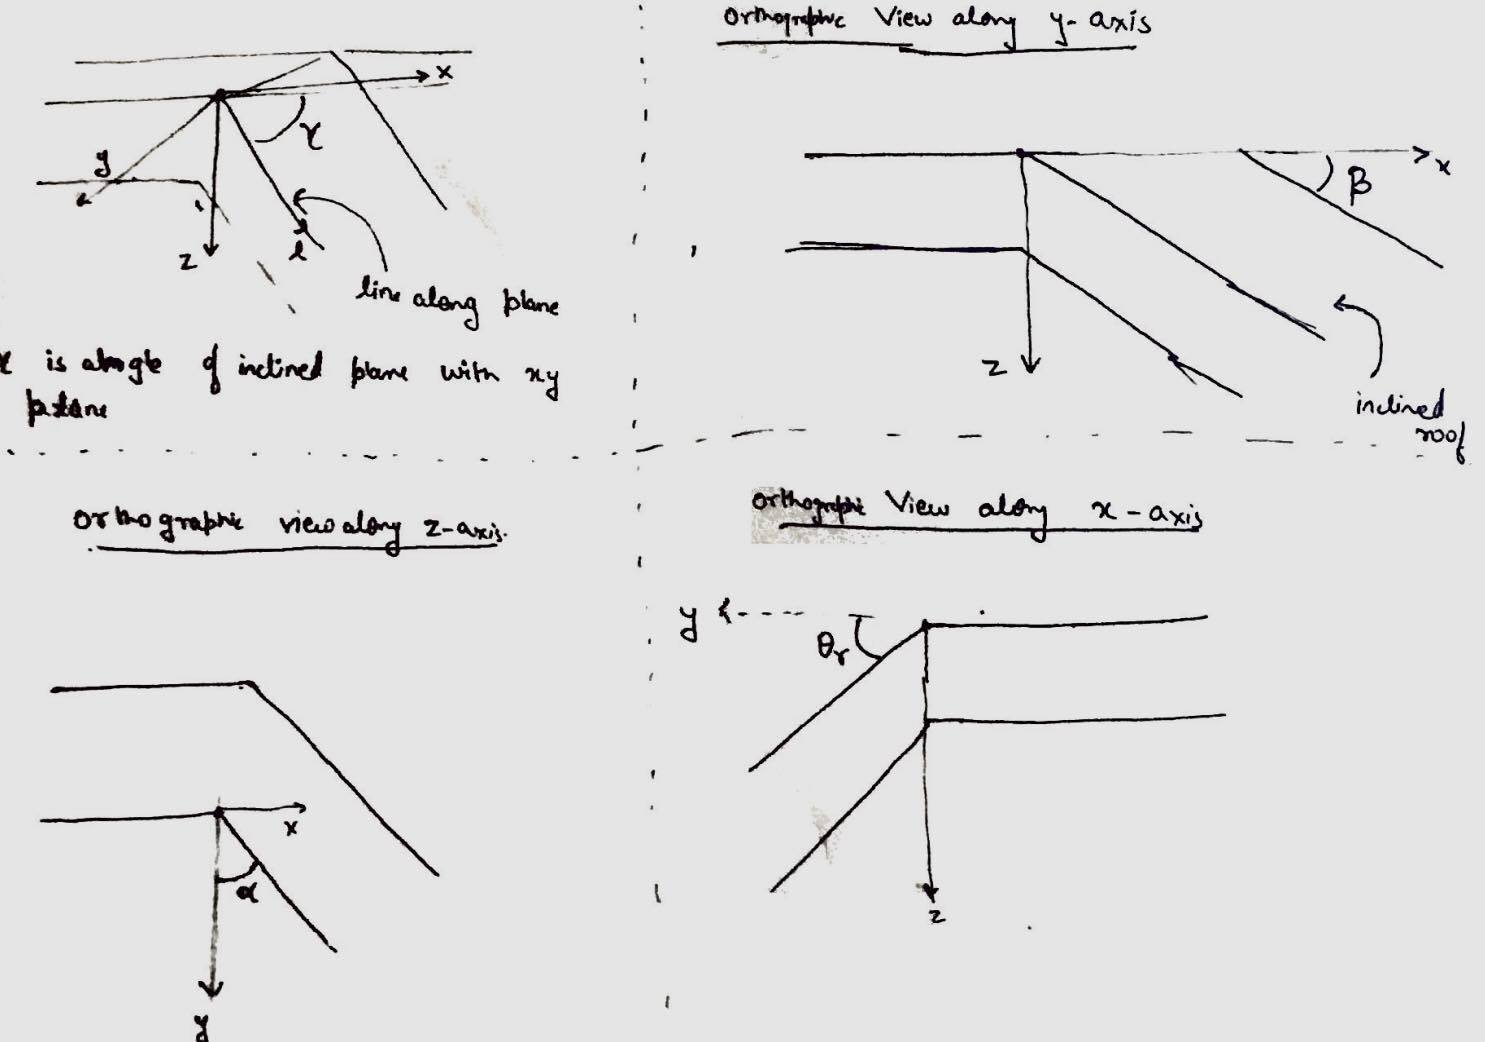
\includegraphics[width=0.8\textwidth]{figures/diagram.jpg}
    \caption{Diagram}
\end{figure*}

\begin{figure*}[ht]!
    \centering
        \begin{subfigure}[ht]{0.475\textwidth}
            \centering
            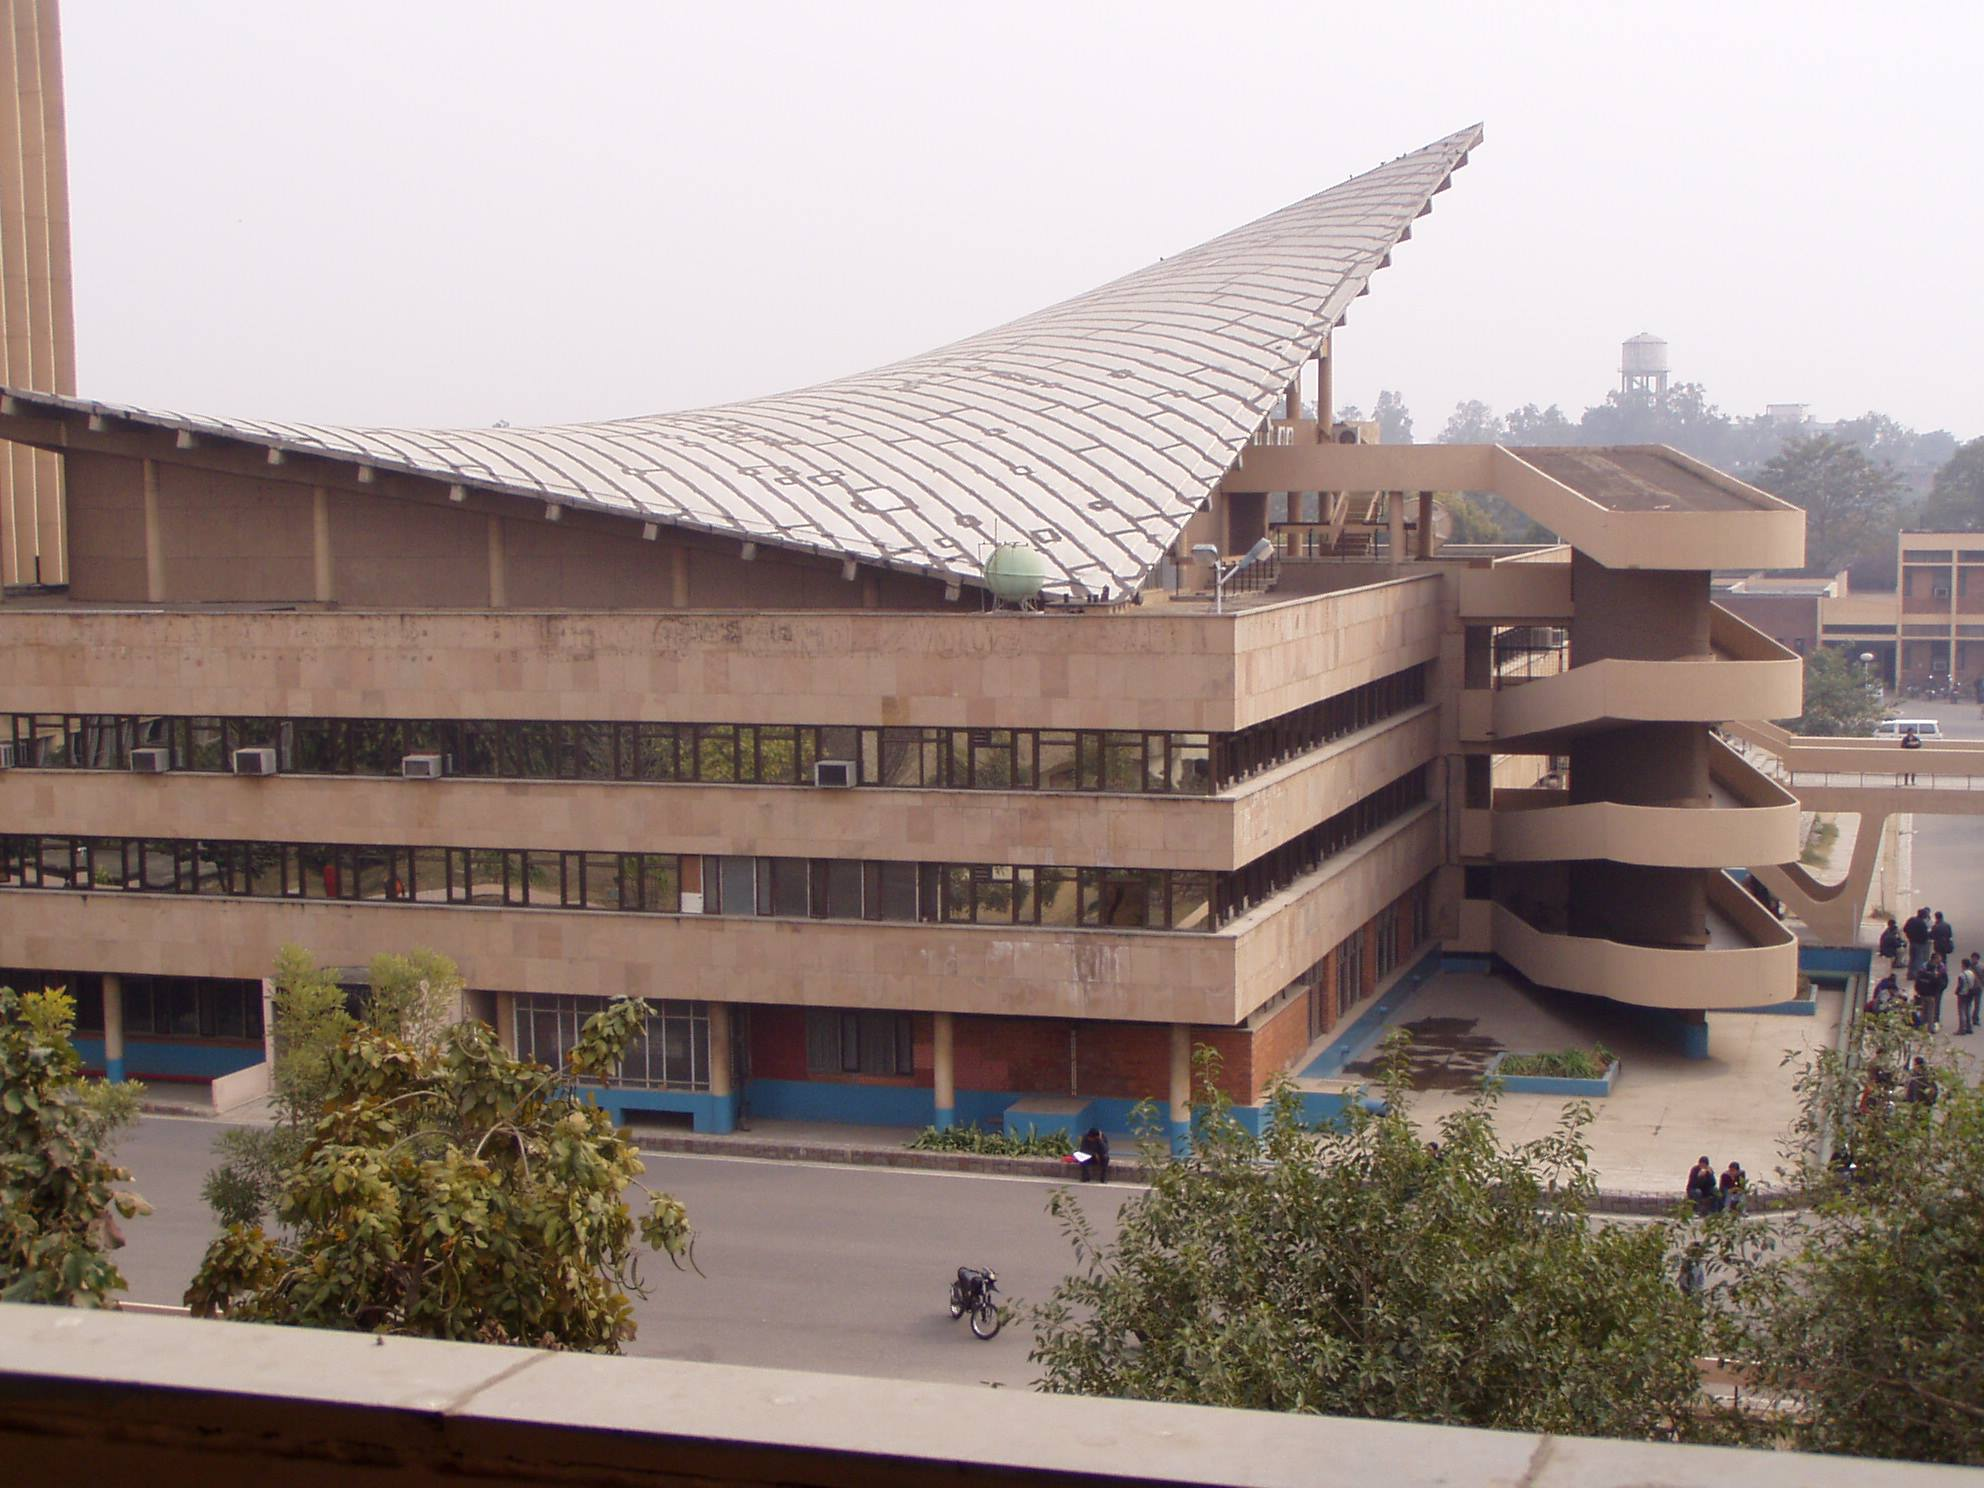
\includegraphics[width=\textwidth]{figures/view.jpg}
            \caption{Staircase\label{fig:staircase}}    
        \end{subfigure}
        \hfill
        \begin{subfigure}[ht]{0.475\textwidth}  
            \centering 
            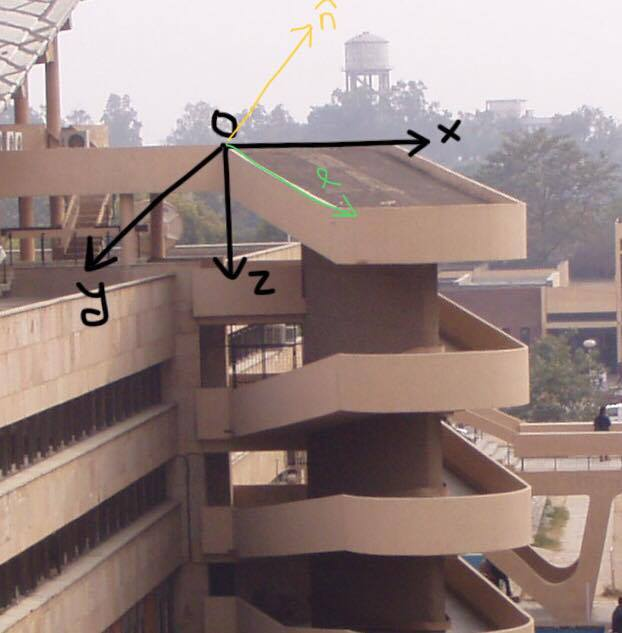
\includegraphics[width=\textwidth]{figures/coordinate.jpg}
            \caption{Coordinate Axis\label{fig:coordinate_axis}}    
        \end{subfigure}
    \vskip \baselineskip
    \centering
        \begin{subfigure}[ht]{0.475\textwidth}   
            \centering 
            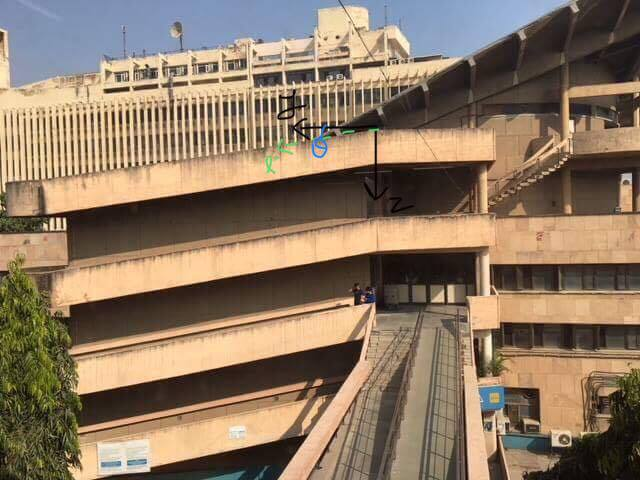
\includegraphics[width=\textwidth]{figures/lib_anno.jpg}
            \caption{Library view\label{fig:lib_anno}}
        \end{subfigure}
        \hfill
        \begin{subfigure}[ht]{0.475\textwidth}  
            \centering 
            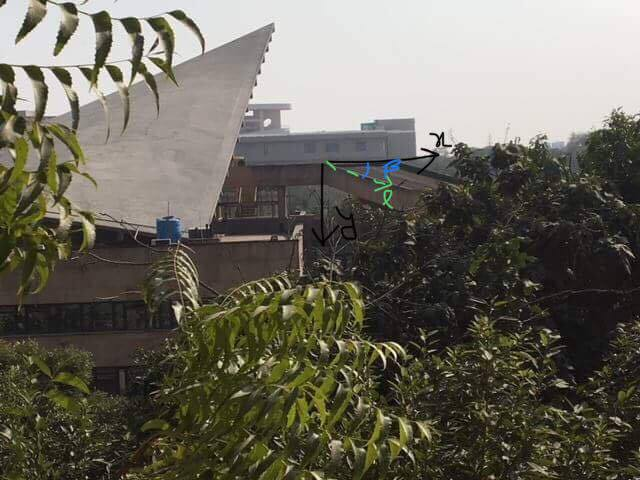
\includegraphics[width=\textwidth]{figures/block_anno.jpg}
            \caption{Block view\label{fig:block_anno}}
        \end{subfigure}
    \caption{Various views used}
\end{figure*}
\pagebreak

\section{Results}
\begin{figure*}[ht]!
    \centering
        \begin{subfigure}[ht]{0.475\textwidth}
            \centering
            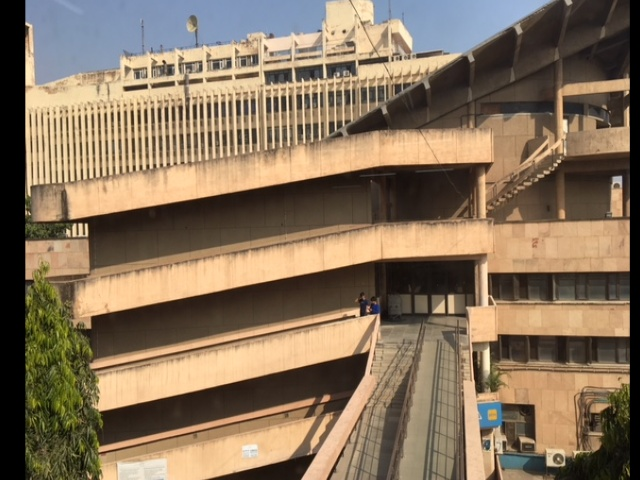
\includegraphics[width=\textwidth]{figures/lib_met.jpg}
            \caption{Metric Corrected library image\label{fig:lib_met}}    
        \end{subfigure}
        \hfill
        \begin{subfigure}[ht]{0.475\textwidth}  
            \centering 
            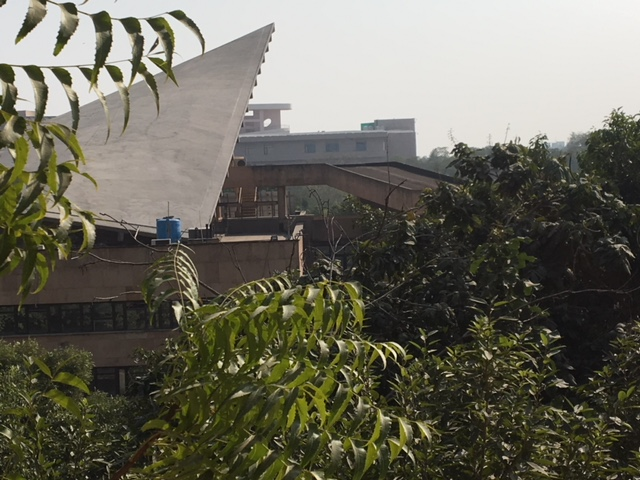
\includegraphics[width=\textwidth]{figures/block.jpg}
            \caption{Metric corrected block image\label{fig:block}}    
        \end{subfigure}
    \vskip \baselineskip
    \caption{Metric correction for the images}
\end{figure*}
We obtained the following results using the orthographic projection method:
\begin{itemize}
    \item $\beta$ = $19.17^o$
    \item $\theta$ = $8.85^o$
    \item $\alpha$ = $24.13^o$
    \item $\gamma$ = $8.08^o$
    \item $n$ = $[0.058, 0.128, -0.99]$
\end{itemize}
The plane has an inclination of $~8^o$ from top of building.

\section*{Declaration of Originality}
I hereby claim that the work presented here is my own and not copied from anywhere. Though, the ideas for the method
were discussed among the following peers: Aman Agrawal (2015CS10210) ,Ankesh Gupta (2015CS10435) and
Saket Dingliwal (2015CS10254), Krunal Shah (2015EE10476).\\
The code that I wrote for the whole process was solely my own.
\end{document}